\chapter{Porównanie wyników algorytmu z komercyjnym rozwiązaniem} 

Systemy biometryczne powinny cechować się dużą skutecznością porównań odcisków, a czas potrzebny na porównanie odcisków powinien być jak najszybszy. Dlatego systemy należy oceniać biorąc pod uwagę właśnie te kryteria. Jakość obu cech jest bardzo istotna. Szybko działający system, dla którego EER\footnote{\em ang. Error equality rate, błąd zrównoważony - błąd, dla progu, dla którego błąd fałszywych odrzuceń i błąd fałszywych dopasowań jest taki sam} jest wysoki jest tak samo nieskuteczny jak bezbłędny system, który obliczenia prowadzi zbyt długo. Ten ostatni można wykorzystać jako wsparcie dla daktyloskopii\footnote{z gr. daktylos – palec i skopeo – patrzę, oglądam) – technika śledcza zajmująca się badaniami porównawczymi linii papilarnych}. Ocena rozwiązania podawana jest na tle komercyjnego programu Fingers Identification Technology\footnote{SDK do porównywania odcisków na licencji Neurotechnology}. Dla potrzeb tej pracy użyto 30 dniowej wersji demonstracyjnej. W zależności od metody porównującej zmieniany jest sposób dopasowywania minucji. Domyślnie SDK posiada swoje wskaźniki obliczające stopień dopasowania, aby porównywanie było miarodajne wykorzystuje ten program jedynie do ekstrakcji minucji i zwrócenia liczby dopasowanych i niedopasowanych minucji. 
\section[Analiza statystyczna kodu][Analiza statystyczna kodu]{Analiza statystyczna kodu} 
Typowym sposobem oceny biometrycznych systemów używających kodowania jako sposobu przetwarzania informacji jest badanie właściwości statystycznych kodu. Dlatego też przeprowadzono porównania w dwóch grupach. Pierwsza z nich dotyczy porównania między odciskami pochodzącymi od tego samego palca. Druga grupa to porównania między różnymi odciskami. W przypadku analizy algorytmu wykonano 2800 porównań. Porównywania wykonywano na zbiorze 800 odcisków, pochodzących od 100 różnych palców, gdzie każdy palec posiada 8 pobranych od niego odcisków. Wybrano dużą liczbe odcisków aby możliwie najlepiej sprawdzic działanie algorytmu. Test wykonywany poprzez porównywanie każdy z każdym wewnątrz odcisków pochodzących od tego samego palca. Druga grupa dotyczy porównania między odciskami pochodzącymi od różnych palców. W przypadku analizy algorytmu wykonano 4950 porównań. Test wykonano na zbiorze 100 odcisków. W tym porównaniu zmniejszono liczbę odcisków, ponieważ nie porównywano odcisków pochodzacych od tego samego palca. Liczba 100 odcisków wystarczyła do wykonania zadowalającej liczby porównań. Jednocześnie mniejsza liczba odcisków jest niewiarygodna dla takiego testu. Porównania wykonano poprzez porównanie każdy - z każdym wewnątrz odcisków pochodzących od różnych palców. Analogiczne testy wykonano dla SDK Neurotechnology. Porównując te same odciski wykonano 300 porównań dla odcisków pochodzących od tego samego palca i 300 dla odcisków pochodzących od różnych. Mała liczba porównań świadczy o tym iż uznano komercyjny program za dość powtarzalny, a testy wykonano dla zgromadzenia wyników na wspólnej bazie odcisków.
\subsection{Rezultaty testów}
\begin{figure}[!hb]
    \begin{center}
		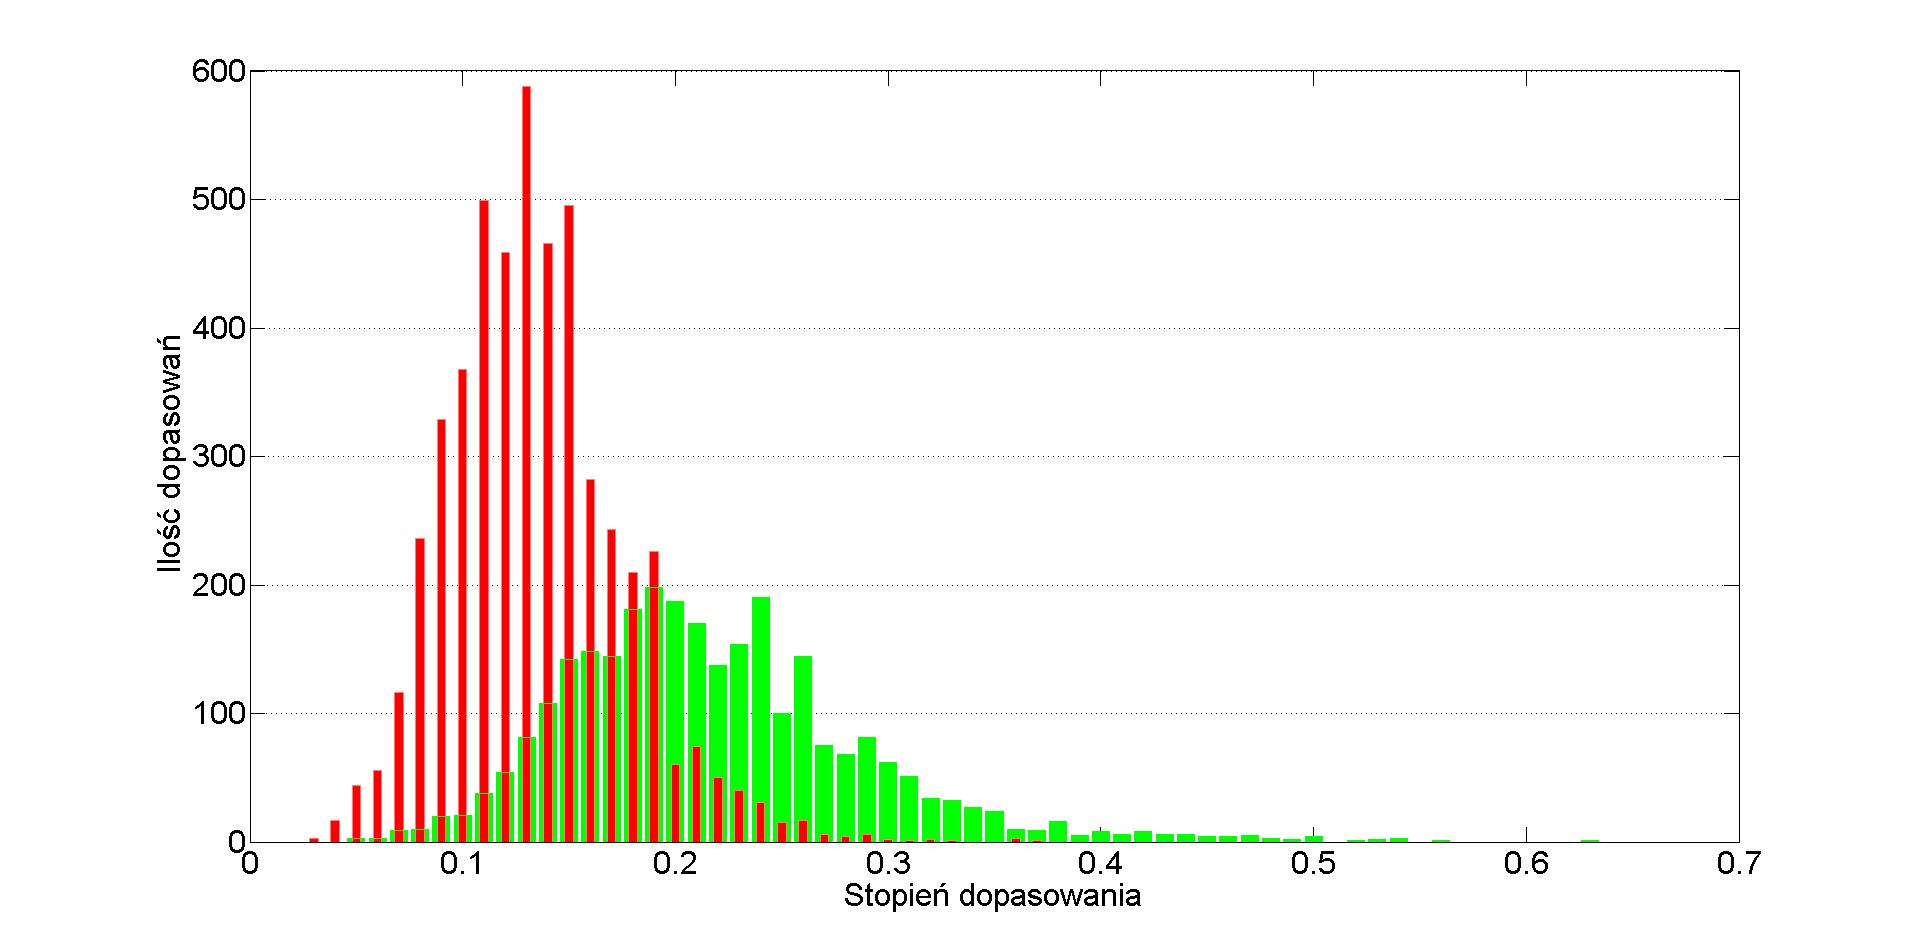
\includegraphics[angle=0,scale=0.27]{img/pattern_bar_statistic_analyses_code_way.jpg}
		\caption{Ilość dopasowań w zależności od jakości dopasowania do odcisku wzorca (test Algorytmu kodowego)}
		\label{img:code_stat_bar_pattern}
    \end{center}
\end{figure} 
Rysunek\ref{img:code_stat_bar_pattern} przedstawia porównania wewnątrz tych samych i różnych odcisków. Kolorem zielonym zaznaczono porównania w grupie tych samych odcisków, czerwonym wewnątrz różnych. Na osi odciętych zaznaczono stopień dopasowania. Jest to iloraz ilości porównań 1:1 do ilości minucji we wzorcu. Świadomie nie stosowano tu klasycznego podejścia odległości Hamminga\footnote{ang. Hamming distance – w teorii informacji jest to wprowadzona przez Richarda Hamminga miara odmienności dwóch ciągów o takiej samej długości}, ponieważ utworzony kod odcisku ma głównie "0", "1" czyli minucje występują w nim rzadko. Zastosowanie odległości Hamminga dawało by wysoką zgodność kodów dla porównywania w obu grupach i wynik byłby nieczytelny. Na osi rzędnych zaznaczono ilość takich dopasowań. Dla czytelności wykres \ref{img:code_stat_line_pattern} przedstawia liniowy sposób reprezentacji poprzedniego wyniku. W dalszej części przedstawiono tylko rysunki liniowe. Wyraźnie widać iż rejony kreślone przez funkcje porównań tych samych i różnych odcisków pokrywają się(miejscie przecięcia zostało zaznaczone niebieską linią). Punk ten wykorzystywany jest do obliczania wskaźników FAR i FRR. Oznacza to, że metoda nie jest pozbawiona błędu. Istnieją odciski które zostaną błędnie zaklasyfikowane jako poprawne oraz te które zostaną błędnie odrzucone. EER dla takiej metody wynosi około 17\%. Oznacza to że przy wyborze progu zaznaczonego niebieską linią co piąte porównanie zostanie błędnie sklasyfikowane. Innowacyjność tej metody porównywania odcisków wskazywałaby na to, że metoda nie koniecznie powinna działać rewelacyjnie. Wynik w granicach 17\% jest jednak wynikiem niedopuszczalnym i przekreśla jakąkolwiek użyteczność tej metody. Dla przedstawionego progu FAR\footnote{ang. False Acceptance Rate -błąd fałszywej akceptacji, ilość odcisków błędnie sklasyfikowanych jako prawdziwe do całości porównywanych odcisków przez system} wynosi nieco ponad 11\%, wiec ok. co dziesiąty odcisk oszusta zostanie zaakceptowany jako prawdziwy. W ustalonym progu FRR\footnote{ang. False Rejection Rate -błąd fałszywego odrzucenia, ilość odcisków błędnie sklasyfikowanych jako nieprawdziwe do całości porównywanych odcisków przez system} wynosi ponad 23\%, oznacza to, że prawie co czwarty prawidłowy odcisk będzie odrzucony. Błąd ten może nie prowadzi do akceptacji próby włamania ale może być uciążliwy dla właściwych użytkowników. Wyobraźmy sobie sytuacje, że ten system zainstalowano w jednym z bankomatów. Więc średnio co 4 wypłata pieniędzy będzie niemożliwa bo system odrzuci nasze logowanie i cały proces należy powtórzyć. Sytuacja wygląda znacznie gorzej gdy system ma zapewniać zerowy błąd akceptacji, wtedy błąd fałszywego odrzucenia wynosi ponad 96\%. Rysunek \ref{img:code_stat_line_sample} pokazuje te same wyniki dla porównywania na tle próbki. Podobnie jak poprzednio wynik do ilość porównań 1:1 do ilości minucji w próbce. Współczynnik EER wzrósł a współczynniki ZERO FRR i ZERO FARi różnią  nieznacznie. Większe różnice występują na poziomie FAR i FRR. Wynika to ze sposobu porównywania odcisków przez algorytm. W skutek dopasowywania kodów algorytm dokręca obrazy odcisków tak aby liczba porównań 0:1 I 1:0 była najmniejsza. Skutkiem ubocznym jest zmniejszanie ilości rozpatrywanych minucji po stronie próbki, dzięki temu liczba rozpatrywanych minucji w próbce jest generalnie mniejsza od liczby minucji we wzorcu. Zmniejszenie ilości minucji po stronie próbki zmniejsza FRR i zwiększa FAR. Dzieje się tak, ponieważ ta sama liczba dopasowanych minucji dzielona przez mniejsza liczbę rozpatrywanych minucji w próbce powoduje przesuwanie wykresu ku większym wartościom. Efekt ten dotyczy zarówno porównań wśród tych samych jak i różnych odcisków, a ponieważ porównania dla odcisków różnych mają mniejszą liczbę trafień niż dla tych samych wykres wykres ten szybciej przesunął się w prawą stronę, a wraz z nim próg EER. Zjawisko to nie występuje dla testów aplikacji $Neurotechnology$ wynika to z innego algorytmu dopasowującego minucje.
\begin{figure}[!ht]
    \begin{center}
		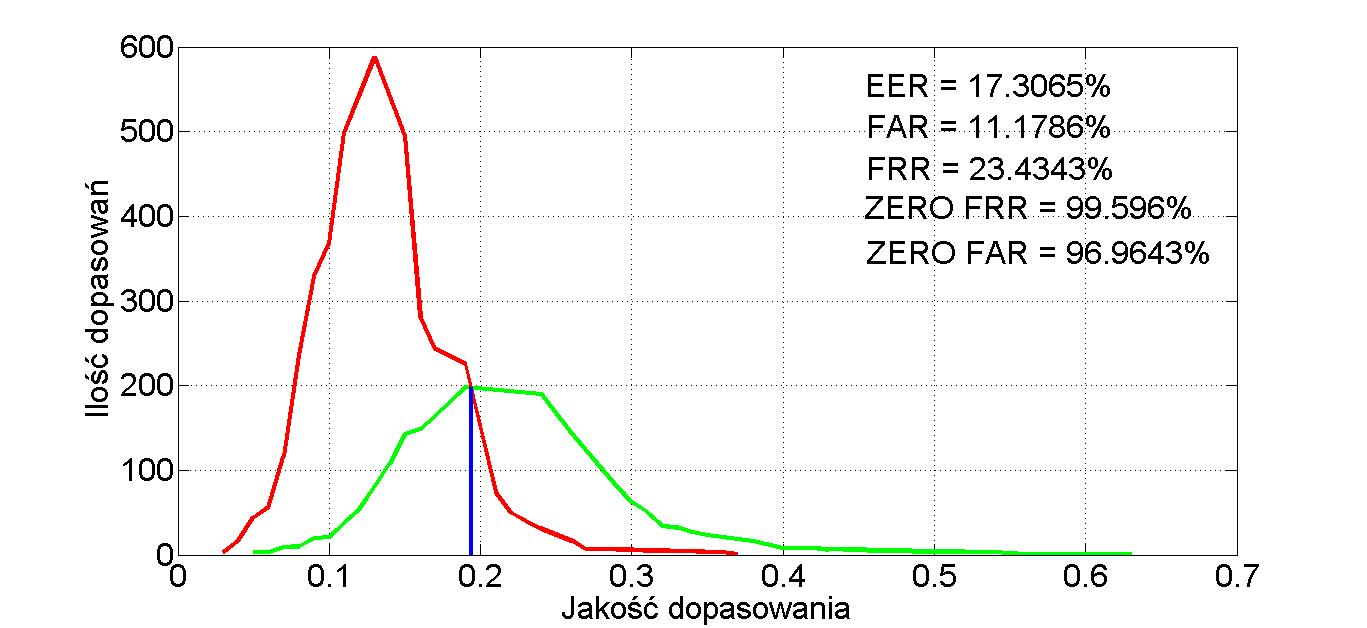
\includegraphics[angle=0,scale=0.27]{img/pattern_line_statistic_analyses_code_way.jpg}
		\caption{Ilość dopasowań w zależności od jakości dopasowania do odcisku wzorca (test Algorytmu kodowego)}
		\label{img:code_stat_line_pattern}
    \end{center}
\end{figure} 

\begin{figure}[!htb]
    \begin{center}
		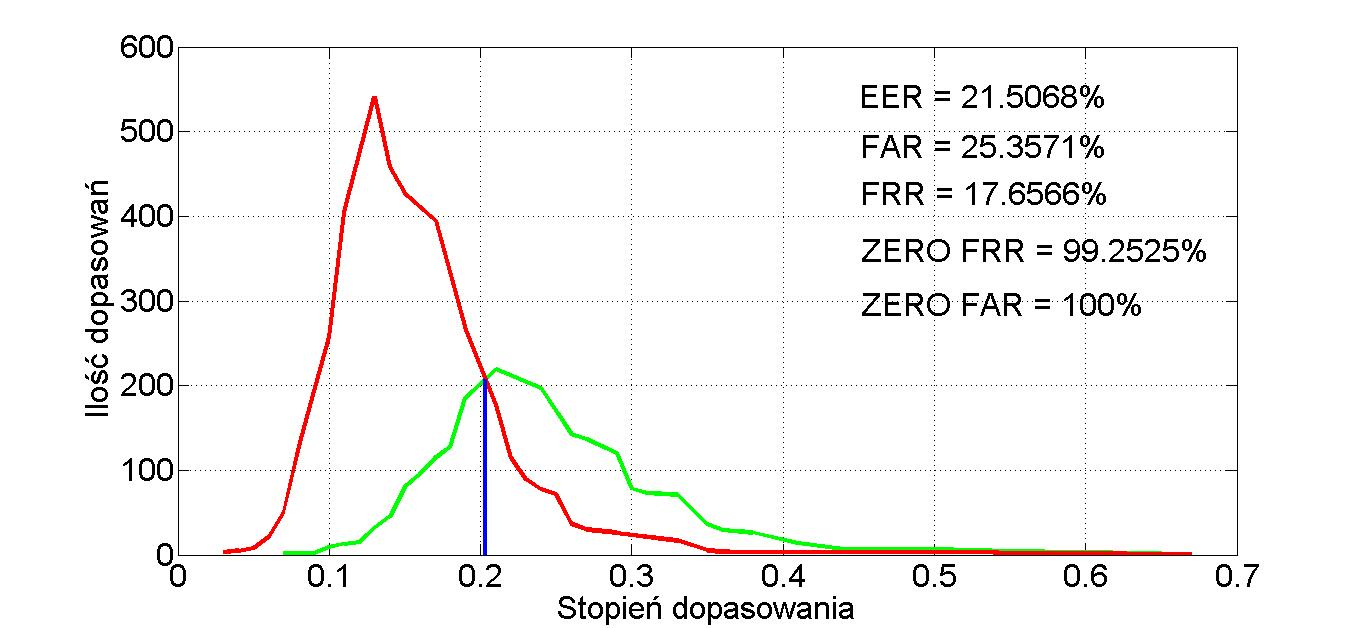
\includegraphics[angle=0,scale=0.27]{img/sample_line_statistic_analyses_code_way.jpg}
		\caption{Ilość dopasowań w zależności od jakości dopasowania do odcisku próbki (test Algorytmu kodowego)}
		\label{img:code_stat_line_sample}
    \end{center}
\end{figure} 
Wyniki przedstawione na tle odcisków próbki są nieznacznie gorsze od wyników przedstawianych na tle wzorca. Wynika to z tego, że algorytm szukając najlepszego dopasowania stosuje transformacje na obrazie próbki, w zależności od dokonanego przekształcenia liczba minucji biorących udział w porównaniu się zmienia mniejsza liczba niedopasowanych minucji może być spowodowana zmniejszeniem się liczby rozpatrywanych minucji próbki. Jest to negatywny skutek uboczny minimalizacji porównań 1:0 i 0:1.
\vspace{.5cm}\par
Komercyjne rozwiązanie wykorzystano w taki sposób aby algorytm porównujący miał zbliżone działanie do przedstawianego kodowania. Wykorzystano jedynie liczbę minucji dopasowanych i nie dopasowanych, generując takie same wykresy. Kolory na wykresach są takie same jak dla testów kodu. Zastosowane metoda nie sugeruje się wskaźnikiem dopasowania zwracanym przez program $Neurotechnology$. Algorytm komercyjny nie korzysta z kodowania odcisku. Wszelkie dopasowania odbywają się przez porównywanie obiektów, a nie kodów. Algorytm komercyjny ma przewagę nad kodowym rozwiązaniem, przechowuje informacje o typie minucji oraz buduje siatkę łącząc dopasowywane minucje. Jest to kolejna informacja, dodatkowo stwierdzająca zgodność dopasowania. Na rysunkach \ref{img:ob_stat_bar_pattern} i \ref{img:ob_stat_line_pattern} zaprezentowano analogiczne do poprzedniego testu wykresy jakości dopasowania względem odcisku wzorca. Rysunki \ref{img:ob_stat_bar_sample} oraz \ref{img:ob_stat_line_sample} prezentują te same wyniki dla próbki. 
\vspace{.5cm}\par
Dla $Neurotechnology$ wynik również nie jest pozbawiony błędu, choć jest o wiele lepszy niż w przypadku zastosowanego algorytmu kodującego. EER dla tej metody wynosi ok 1.5\%, mimo iż jest 10 krotnie mniejszy niż dla kodu odcisku,  nie zapewnia należytej ochrony wymaganej od systemów biometrycznych. Warto zauważyć, iż podawany wynik nie dotyczy skuteczności oprogramowania $Neurotechnology$, a jedynie jego udziału w proponowanym sposobie porównywania odcisków. Zdecydowanie lepiej wypadają też współczynniki FAR i FRR, które wynoszą odpowiednio ok 1\% i 2\%. Natomiast znacznie lepiej prezentuje się w przypadku błędów zerowych. Wystarczy zaakceptować błąd w granicach 7\% i system stanie się bezbłędny. Oczywiście wyniki dotyczą tylko bazy danych na której był przeprowadzany test. Przeprowadzany test dowodzi, iż kodowa metoda porównywania odcisków dopasowuje odciski znacznie gorzej niż metoda obiektowa. Dodatkowo porównywanie jedynie liczby minucji pasujących nie wystarcza do jednoznacznego stwierdzenia podobieństwa bądź niepodobieństwa obrazów. Kolejną wadą przedstawianego rozwiązania jest brak porównań dla których jest 100\% zgodność lub analogiczna niezgodność. Wynika to z doboru parametrów, a zwłaszcza wielkości kratki kodu. Zmniejszenie kratki powodowało pojawianie się porównań o 100\% niezgodności natomiast zwiększanie sprzyja łatwiejszemu dopasowywaniu kodów. Niestety ustawienia te źle wpływały na ilość poprawnych porównań. Ustawienie optymalnej wielkości kratki powoduje zmniejszenie liczby całkowitych zgodności i niezgodności.

\begin{figure}[!hbt]
    \begin{center}
		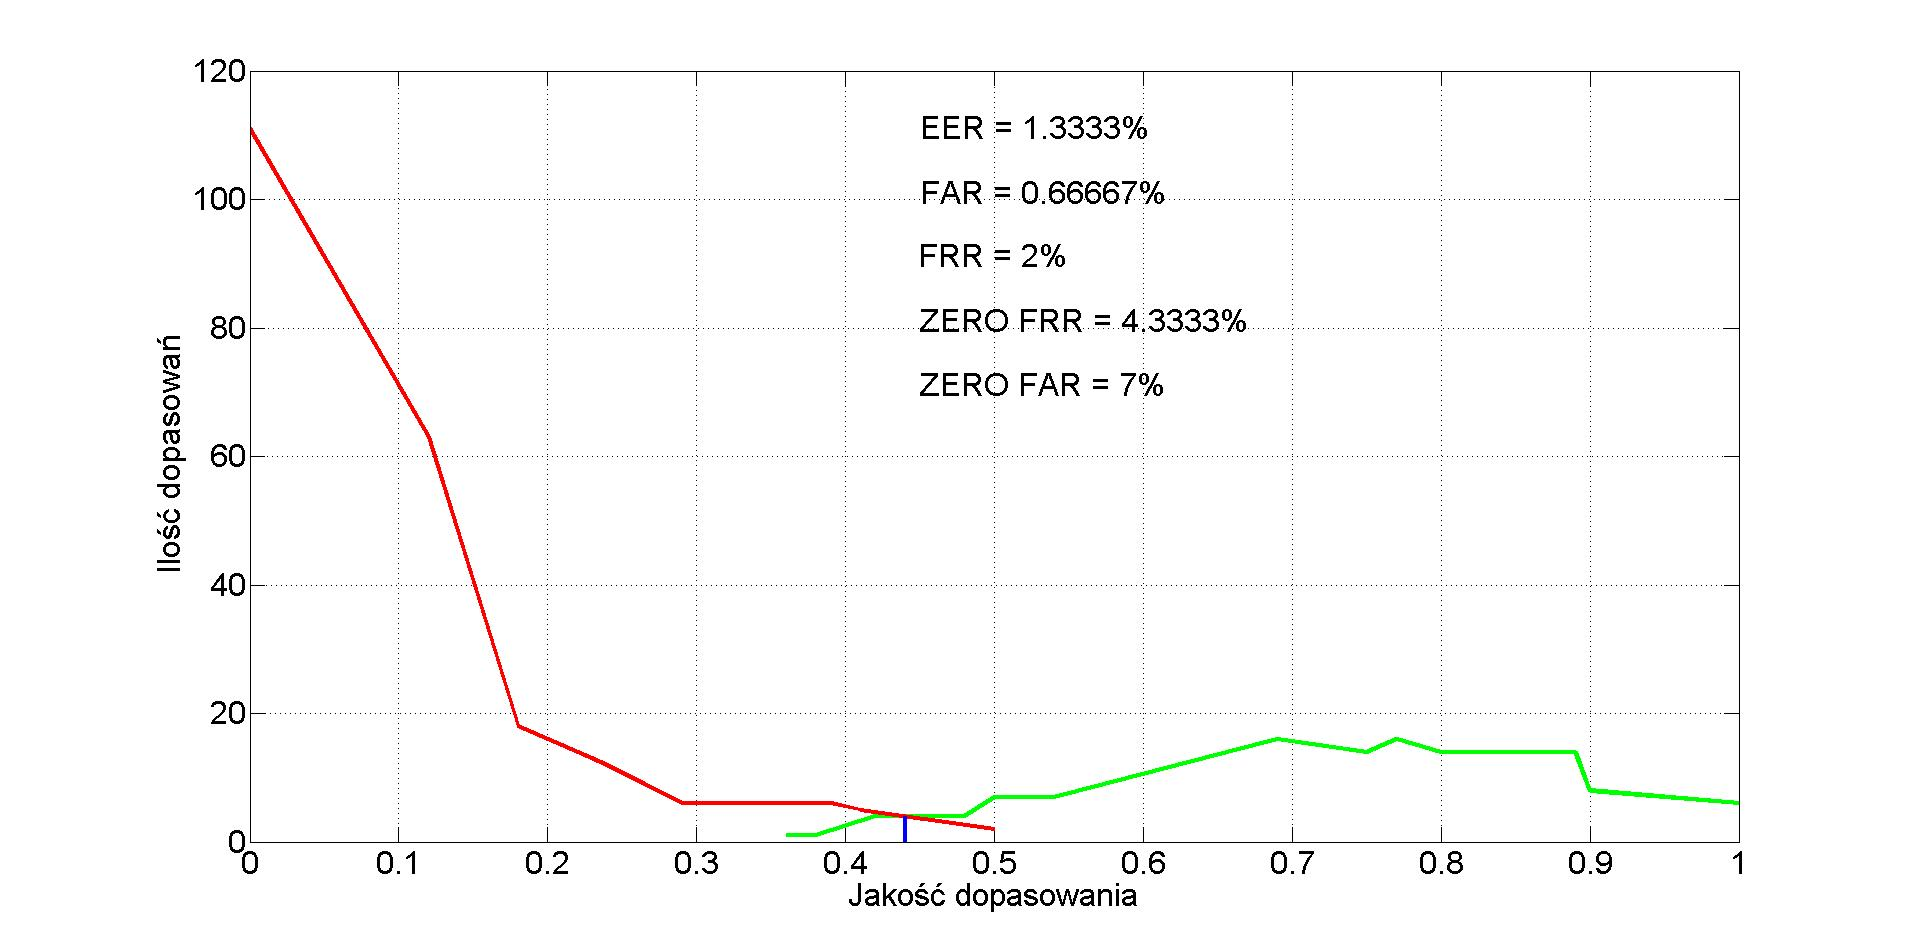
\includegraphics[angle=0,scale=0.27]{img/pattern_line_statistic_analyses_ob_way.jpg}
		\caption{Ilość dopasowań w zależności od jakości dopasowania do odcisku wzorca (test $Neurotechnology$)}
		\label{img:ob_stat_line_pattern}
    \end{center}
\end{figure} 
\newpage 

\begin{figure}[!hbt]
    \begin{center}
		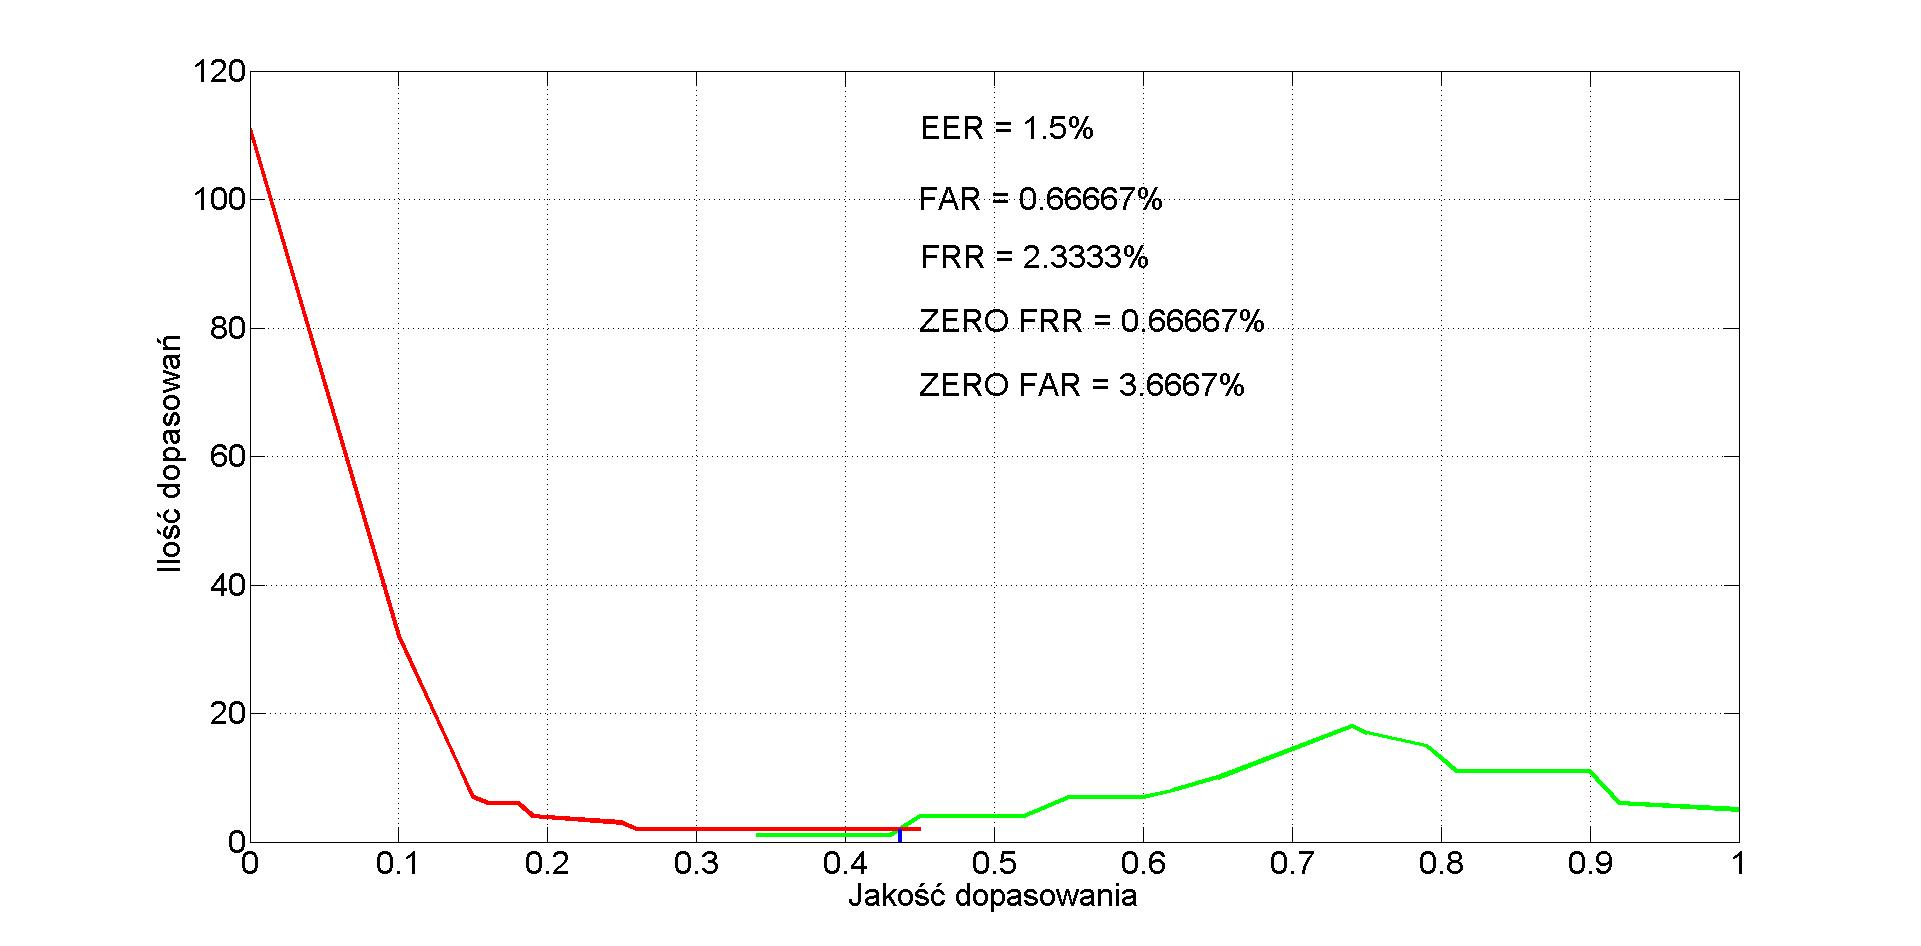
\includegraphics[angle=0,scale=0.27]{img/sample_line_statistic_analyses_ob_way.jpg}
		\caption{Ilość dopasowań w zależności od jakości dopasowania do odcisku próbki (test $Neurotechnology$)}
		\label{img:ob_stat_line_sample}
    \end{center}
\end{figure} 

\newpage 
\section[Rozkład punktów porównania][Rozkład punktów porównania]{Rozkład punktów porównania}

Przeprowadzone testy dowodzą jednoznacznie, że sposób porównywania tylko liczby zgodnych minucji nie wystarcza do stwierdzenia poprawnego podobieństwa lub nie podobieństwa obrazów. Choć metoda ta jest jedną z głównych metod stwierdzających prawidłowe dopasowanie odcisków to dla wykorzystań opisywanego algorytmu jest całkowicie zawodna. Przyczyn może być wiele
\renewcommand*{\labelitemi}{\bullet}
\begin{itemize}
\item Błąd algorytmu
\item Błąd implementacji
\item Niewystarczająca ilość kodowanej informacji
\item Zbytnie uproszczenie kodowanej informacji
\item Brak filtrowania minucji, chodzi tu o odrzucanie minucji o niewystarczającej jakości
\item Błąd sposobu porównania kodów
\end{itemize}
Przyczyny związane z błędami w kodzie programu odrzucam, gdyż testy aplikacji dowodzą prawidłową realizację wymyślonego algorytmu. Błąd algorytmu stawiałby poważną barierę w rozwoju tego typu podejścia dlatego dla celów badawczych również jest tu pomijany. Zwiększenie ilości kodowanej informacji mogłoby przekształcić algorytm kodowania w inny zapis algorytmu obiektowego. Naturalne wydaje się iż w algorytmach tworzących kod jakiejś próbki biometrycznej wartości cech biometrycznych są uśredniane i wynik ten nie powinien przeszkadzać w porównywaniu obrazów. Dowodem tego może być algorytm Dougman-a do kodowania tęczówki oka. Obraz tęczówki jest świadomie uśredniany, a mimo wszystko nie przeszkadza to w dalszej identyfikacji. trafnym pomysłem jest odrzucanie minucji o złej jakości. W procesie przetwarzania obrazu znalezione współrzędne niekoniecznie muszą wyznaczać minucje odcisku. Nikt nie gwarantuje wysokiej jakości obrazu z czytnika. Dlatego znalezione punkty mogą być tylko zakłóceniem obrazu a nie rzeczywistą minucją. Mimo tego rozwiązanie to nie zostało zastosowane. Powodem jest rożna interpretacja minucji przez różne SDK'i do ekstrakcji minucji z obrazu. Metoda musi być  niezależna od sposobu zdobywania minucji dlatego nie powinno polegać się na wskazaniach SDK'a. Zawsze można zastosować inne oprogramowanie. Metoda zmiany SDK nie jest metodą naprawy błędu omawianego rozwiązania. Jedynym zatem rozważanym sposobem poprawy jest zmiana sposobu porównywania już zakodowanych odcisków. Pierwotnie wzorem istniejących metod największy nacisk położony jest na liczbę dopasowanych minucji. Dlatego proponowanym wyjściem jest zastosowanie różnicy symetrycznej czyli liczby niedopasowanych minucji po stronie wzorca i liczby niedopasowanych minucji po stronie próbki. Są to dane obecnie nie wykorzystywane w procesie porównywania. Rozwiązanie to zostało szerzej omówione w rozdziale 5. Innym sposobem jest wykorzystanie wszystkich 3 rodzajów porównań i w zależności od ich liczby decydować czy odciski należą do tej samej osoby czy do różnych. Możliwe jest to poprzez zastosowanie wag dla każdego z tych porównań przyjmując przykładowo 1 punkt za porównanie 1:1 i -1 punkt za porównania 0:1 i 1:0. Rozwiązanie to jest jednak wrażliwe na sumę minucji w próbce i we wzorcu otrzymane ilości punktów będą więc różnić się w zależności od odcisków jakie będą porównywane. Zastosowanie takiej metody wymagało by stworzenie tablicy progów zamiast jednego globalnego progu separującego odciski.
\subsubsection{Przykład 1}
Dane są cztery odciski po dwa od osoby A i B. Posiadają odpowiednio 30, 25 minucji dla osoby A oraz 12, 15 minucji osoby B. Porównując dwa odciski osoby A otrzymano 15 minucji zgodnych, porównując odciski osoby B otrzymano 8 odcisków zgodnych. Porównania między osobami A(30) i B(12) dają 6 odcisków zgodnych. Gdyby wyliczać współczynniki porównania w podany powyżej sposób dla porównania wewnątrz tych samych osób otrzymano wynik -10 i -3 punkty. Porównanie między osobami A i B daje wynik -30 pkt

\subsubsection{Przykład 2}
Dane są dwa odciski po jednym od osoby A i B. Posiadają odpowiednio 30 i 40 minucji. Porównania między osobami A(30) i B(40) dają 15 odcisków zgodnych. Ten sam sposób wyliczeń współczynników dla porównania daje wynik -40 pkt. 
\vspace{.5cm}\par
Przykład 1 prezentuje udaną próbę zastosowania zmienionego systemu porównań, jeżeli za próg separujący przyjmiemy liczbę z przedziału (-3; -30). Przykład 2 prezentuje porównanie które powinno być potraktowane jako niezgodne, natomiast dla progu z przykładu 1 zaklasyfikowane zostanie przez system jako zgodne. Te dwa proste przykłady prezentują ogromną wrażliwość przedstawionego rozwiązania. Można oczywiście zakładać iż przedstawione wyniki nie będą odzwierciedlać prawdziwej sytuacji. Jednak dla testowanej bazy danych liczba minucji dla jednego palca waha się od 14 do 51 minucji, więc gdyby dwa odciski o względnie dużej liczbie minucji i dość gęstym ustawieniu porównać testowanym algorytmem możliwe jest uzyskanie zgodności nawet większej od 10 minucji. Proste punktowanie nie uwzględnia jednak liczby minucji we wzorcu i w próbce. Dokonano doświadczenia i narysowano rozkład punktów porównań w przestrzeni przyjmując jako współrzędne XYZ punkty odpowiadające liczności porównań (1:1), (1:0) i (0:1) dla całej pary próbka wzorzec. Rozkład punktów przedstawia rysunek \ref{img:cloud_all}, natomiast rzuty na poszczególne dwuwymiarowe przestrzenie przedstawiają rysunki \ref{img:cloud_1}, \ref{img:cloud_2}, \ref{img:cloud_3}. Podobnie jak poprzednio kolorem zielonym zaznaczono punkty dla porównań między odciskami należącymi do tych samych palców, czerwonym dla różnych. Wykres potwierdza przypuszczenia o różnym rozłożeniu punktów w przestrzeni. Niestety żaden rzut na przestrzenie dwuwymiarowe nie zapewnia separacji tych punktów. Szersze zastosowanie tej metody porównania omówione zostało w rozdziale 6.

\begin{figure}[!hbt]
    \begin{center}
		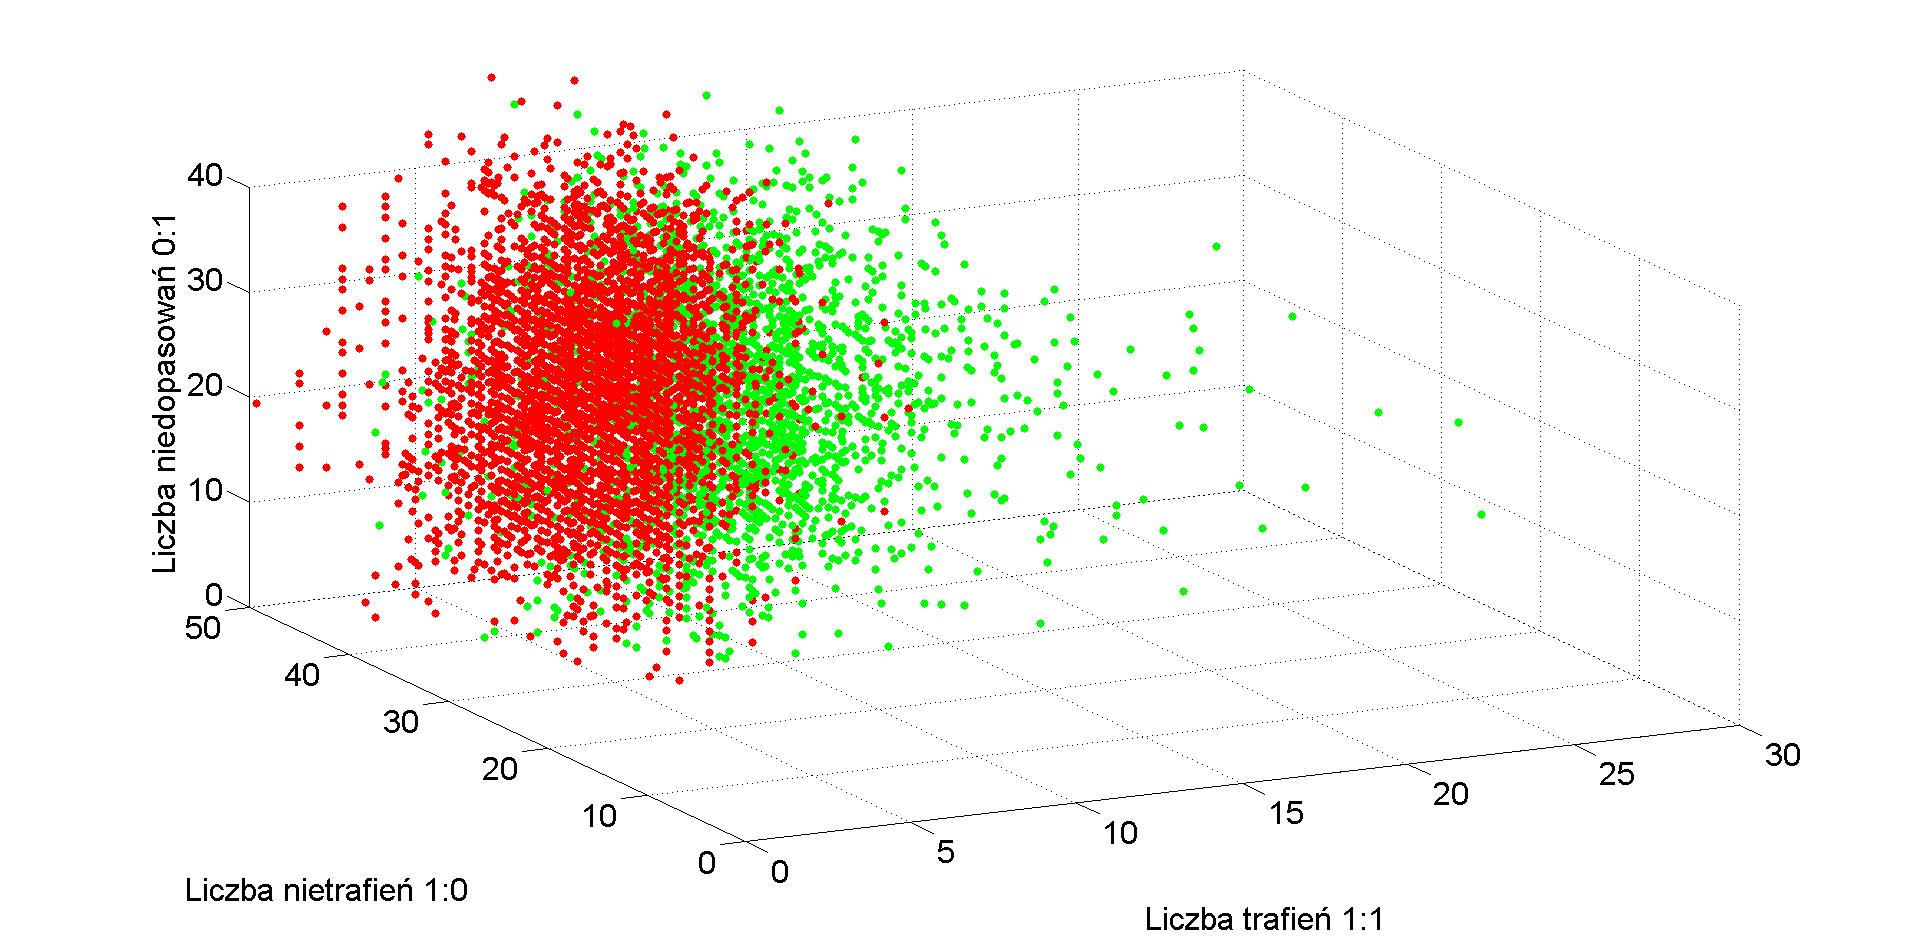
\includegraphics[angle=0,scale=0.27]{img/cloud.jpg}
		\caption{Rozkład punktów dopasowań dla porównań kodów odcisku}
		\label{img:cloud_all}
    \end{center}
\end{figure} 

\begin{figure}[!hbt]
    \begin{center}
		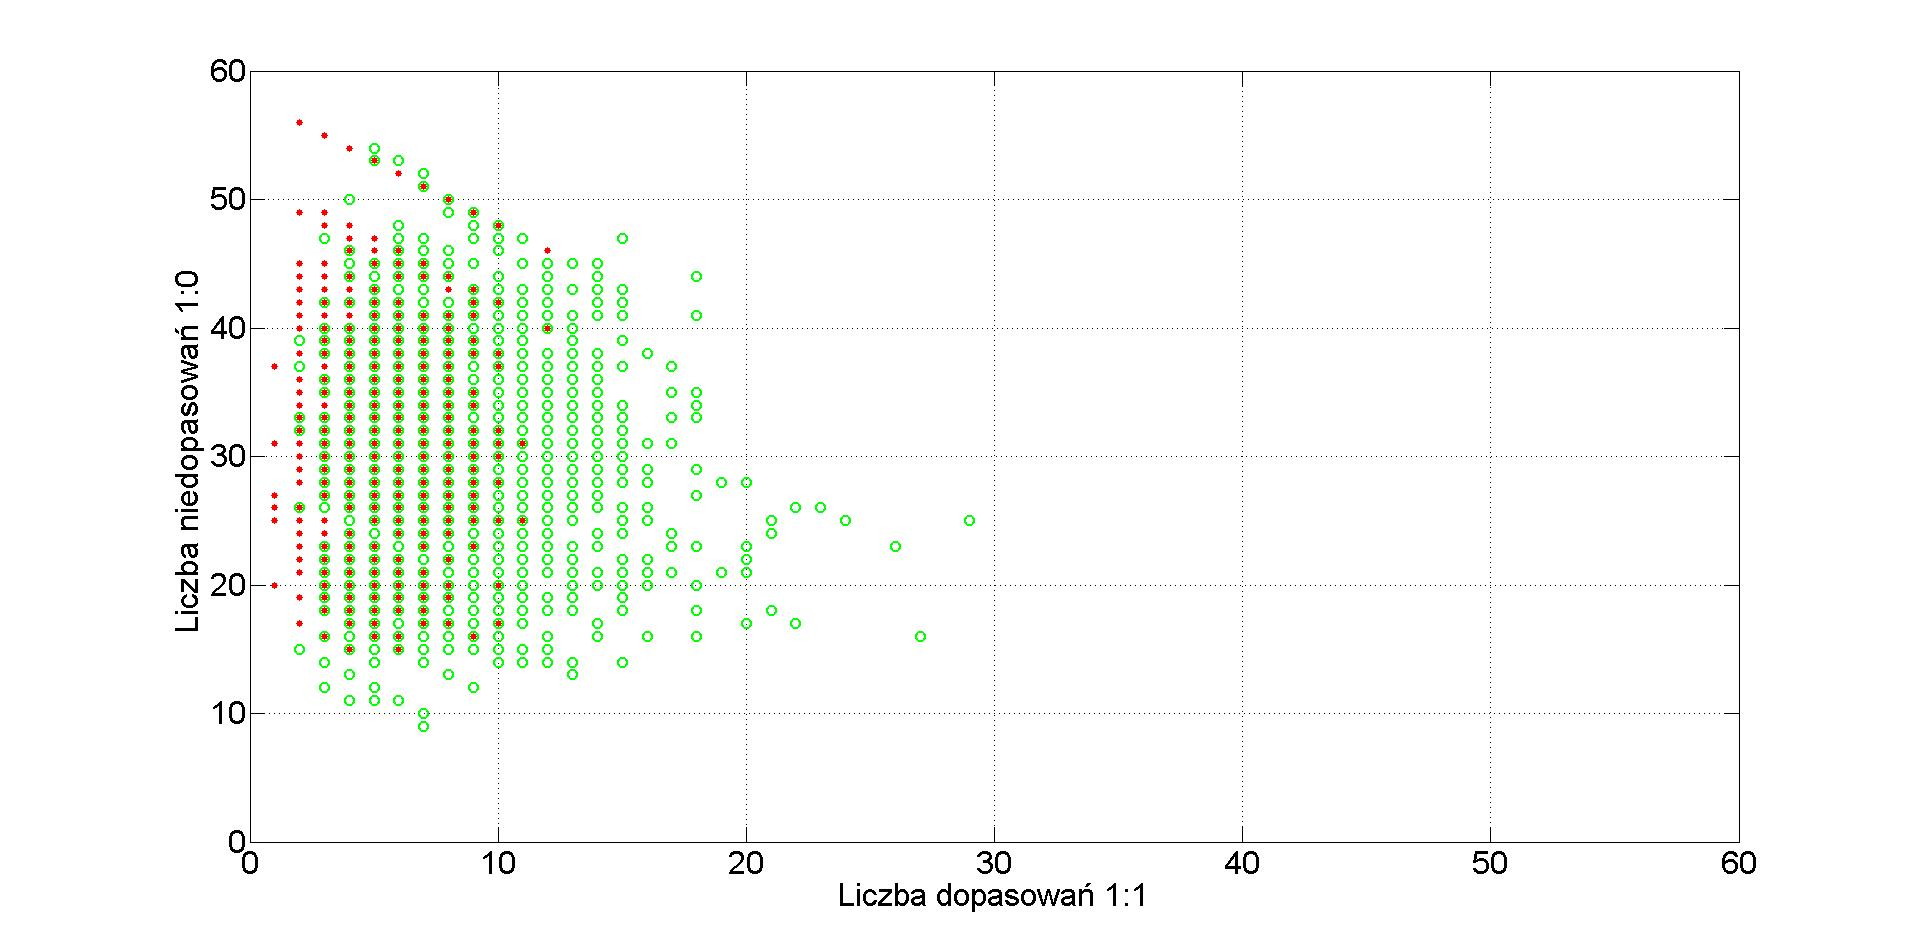
\includegraphics[angle=0,scale=0.27]{img/cloud_1.jpg}
		\caption{Rozkład punktów dopasowań dla porównań kodów odcisku na przestrzeni porównań (1:1) (1:0)}
		\label{img:cloud_1}
    \end{center}
\end{figure} 

\begin{figure}[!hbt]
    \begin{center}
		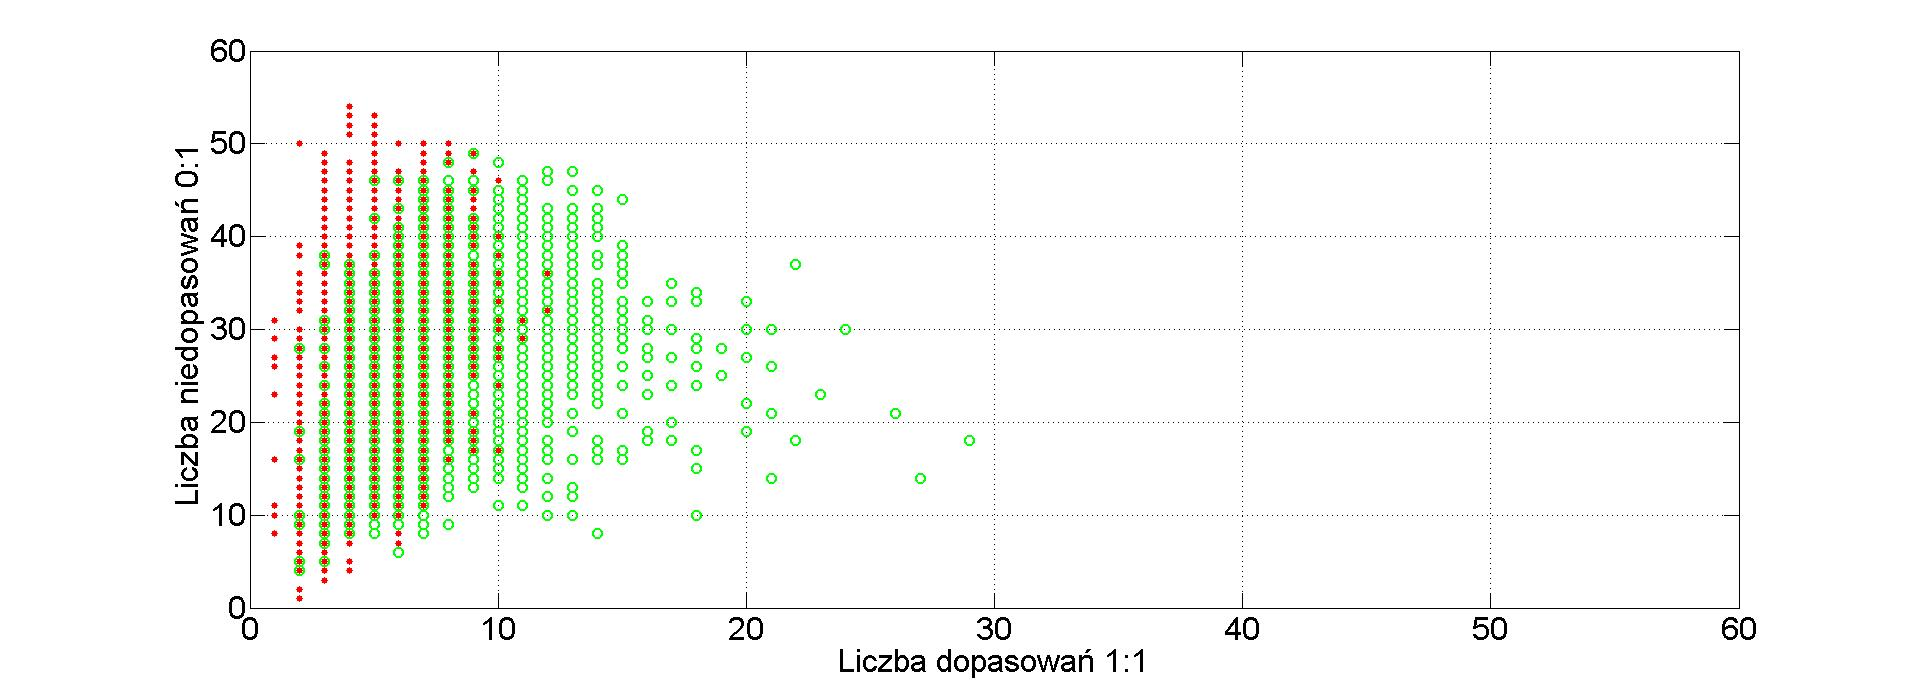
\includegraphics[angle=0,scale=0.27]{img/cloud_2.jpg}
		\caption{Rozkład punktów dopasowań dla porównań kodów odcisku na przestrzeni porównań (1:1) (0:1)}
		\label{img:cloud_2}
    \end{center}
\end{figure} 

\begin{figure}[!hbt]
    \begin{center}
		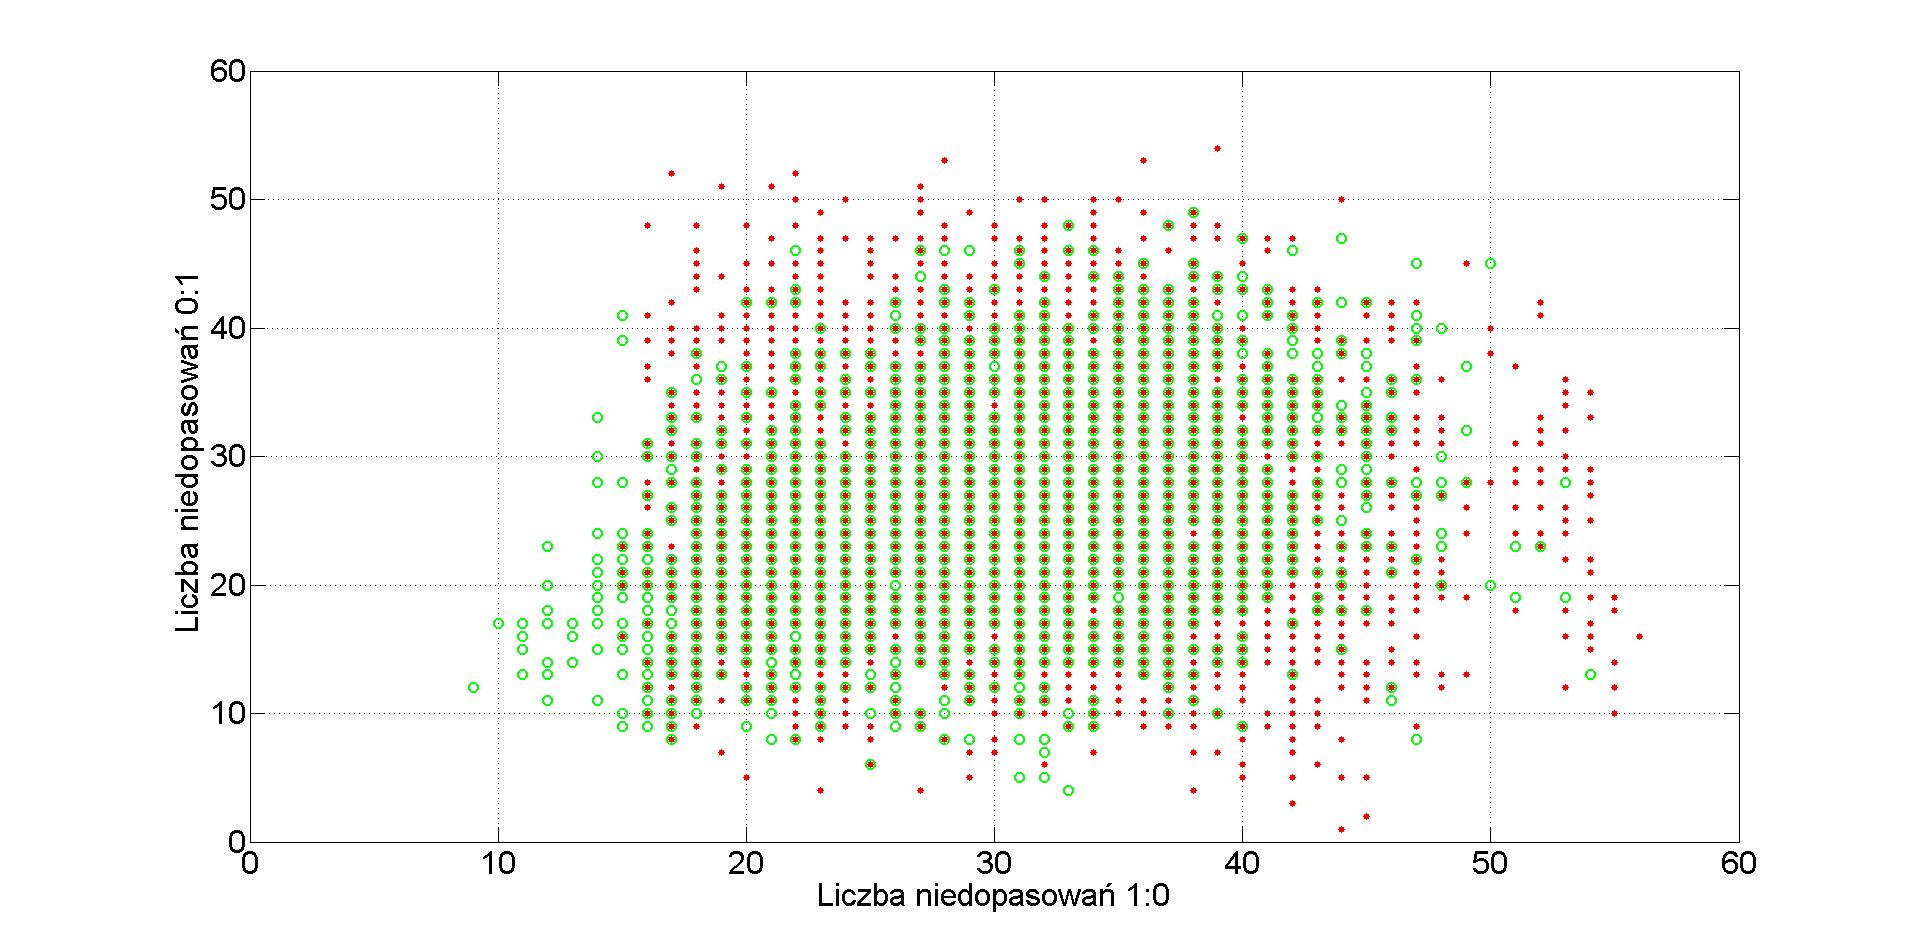
\includegraphics[angle=0,scale=0.27]{img/cloud_3.jpg}
		\caption{Rozkład punktów dopasowań dla porównań kodów odcisku na przestrzeni porównań (1:0) (0:1)}
		\label{img:cloud_3}
	\end{center}
\end{figure} 